% =====================================================================
%  Chapitre 2 -- Preparer les donnees sans se tromper
%  Partie a : manquants, imputation, encodage  (Licence 3 SDIA)
% =====================================================================
\section{Chapitre 2 --- Préparer les données}

\chapterslide{Chapitre 2}{Préparer les données sans se tromper}%
{4 h --- 2 h CM/TD + 2 h TP}%
{\textbf{Objectifs.} Traiter les valeurs manquantes sans biaiser ; encoder les
variables catégorielles ; choisir une mise à l'échelle ; placer tout le
prétraitement dans un pipeline.}

\begin{frame}{Le modèle ne voit que ce qu'on lui donne}
\begin{columns}[t]
\begin{column}{0.48\textwidth}
\begin{ebox}[Ce que reçoit le modèle]
Un tableau de nombres. Ni les unités, ni le sens des colonnes, ni les
modalités : seulement des valeurs.
\end{ebox}
\end{column}
\begin{column}{0.48\textwidth}
\begin{wbox}[Ce que cela implique]
Une colonne mal encodée, une échelle absente ou une imputation faite au
mauvais moment, et le meilleur modèle du monde produira un résultat faux.
\end{wbox}
\end{column}
\end{columns}
\vspace{2mm}
\begin{center}
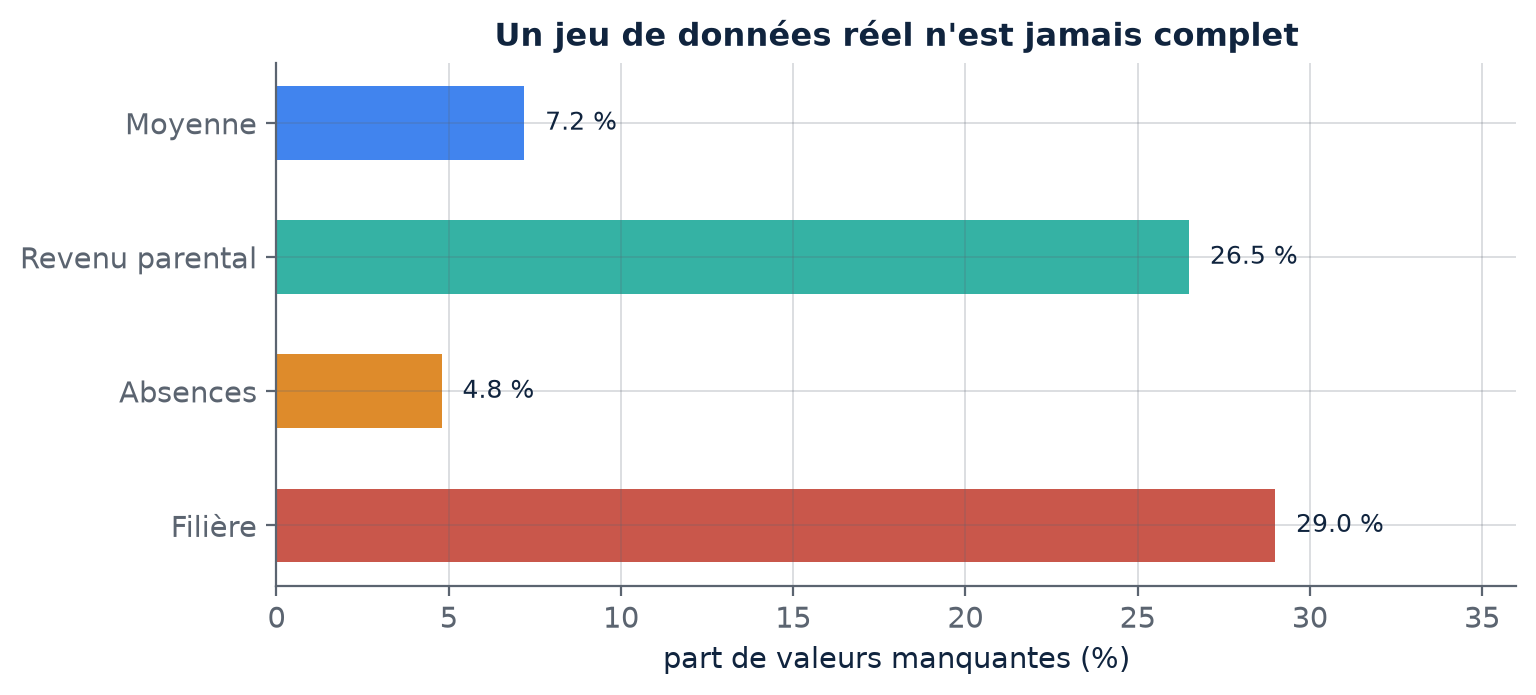
\includegraphics[width=0.90\textwidth]{h01_manquants.png}
\end{center}
\end{frame}

\begin{frame}{Quatre défauts que tout jeu réel présente}
\begin{center}
\small
\begin{tabular}{@{}p{0.22\textwidth}p{0.30\textwidth}p{0.36\textwidth}@{}}
\toprule
\textbf{Défaut} & \textbf{Exemple} & \textbf{Risque si on l'ignore} \\
\midrule
Valeurs manquantes & revenu parental absent (26,5 \%) & le modèle refuse, ou
apprend un motif artificiel \\
Échelles hétérogènes & âge (0--100) et revenu (0--500\,000) & les distances
sont dictées par la plus grande colonne \\
Catégories en texte & « Informatique », « Télécom » & impossible à calculer
tel quel \\
Valeurs aberrantes & température 1\,575 °C & la moyenne et les coefficients
sont tirés \\
\bottomrule
\end{tabular}
\end{center}
\vspace{1.5mm}
\begin{kbox}[Ordre de travail]
On traite les défauts \textbf{avant} d'entraîner, mais on les traite
\textbf{dans} le pipeline. Les deux phrases ne se contredisent pas : voir la
fin du chapitre.
\end{kbox}
\end{frame}

\begin{frame}{Valeurs manquantes : trois mécanismes}
\begin{center}
\small
\begin{tabular}{@{}p{0.14\textwidth}p{0.34\textwidth}p{0.40\textwidth}@{}}
\toprule
\textbf{Sigle} & \textbf{Signification} & \textbf{Conséquence} \\
\midrule
MCAR & manque \textbf{complètement au hasard} (capteur en panne) & on peut
supprimer ou imputer sans biais majeur \\
MAR & le manque dépend d'une \textbf{autre variable observée} (les hauts
revenus refusent de répondre) & imputation conditionnelle possible \\
MNAR & le manque dépend de la \textbf{valeur elle-même} (les très hauts
revenus ne répondent jamais) & biais non corrigeable sans information
externe \\
\bottomrule
\end{tabular}
\end{center}
\vspace{1.5mm}
\begin{wbox}[À retenir]
Avant de choisir une méthode, demandez-vous \emph{pourquoi} la valeur manque.
La réponse détermine si l'imputation est légitime ou si elle fabrique un
résultat.
\end{wbox}
\end{frame}

\begin{frame}{Supprimer ou imputer ?}
\begin{columns}[t]
\begin{column}{0.48\textwidth}
\begin{ebox}[Supprimer]
\begin{itemize}
  \item lignes incomplètes : acceptable si $<5\,\%$ et MCAR ;
  \item colonnes trop incomplètes ($>50\,\%$) ;
  \item jamais : supprimer les lignes d'une classe rare.
\end{itemize}
\end{ebox}
\end{column}
\begin{column}{0.48\textwidth}
\begin{ebox}[Imputer]
\begin{itemize}
  \item \textbf{médiane} : robuste aux valeurs extrêmes ;
  \item \textbf{moyenne} : seulement si la distribution est symétrique ;
  \item \textbf{KNN} ou modèle : exploite les autres colonnes ;
  \item ajouter une colonne « était manquant » si le manque est informatif.
\end{itemize}
\end{ebox}
\end{column}
\end{columns}
\vspace{1.5mm}
\begin{kbox}[Le piège de l'imputation par la moyenne]
Elle conserve la moyenne, mais elle \textbf{écrase la variance} : les valeurs
imputées s'accumulent au centre. La distribution n'est plus la même.
\end{kbox}
\end{frame}

\begin{frame}{Ce que l'imputation fait vraiment à vos données}
\begin{center}
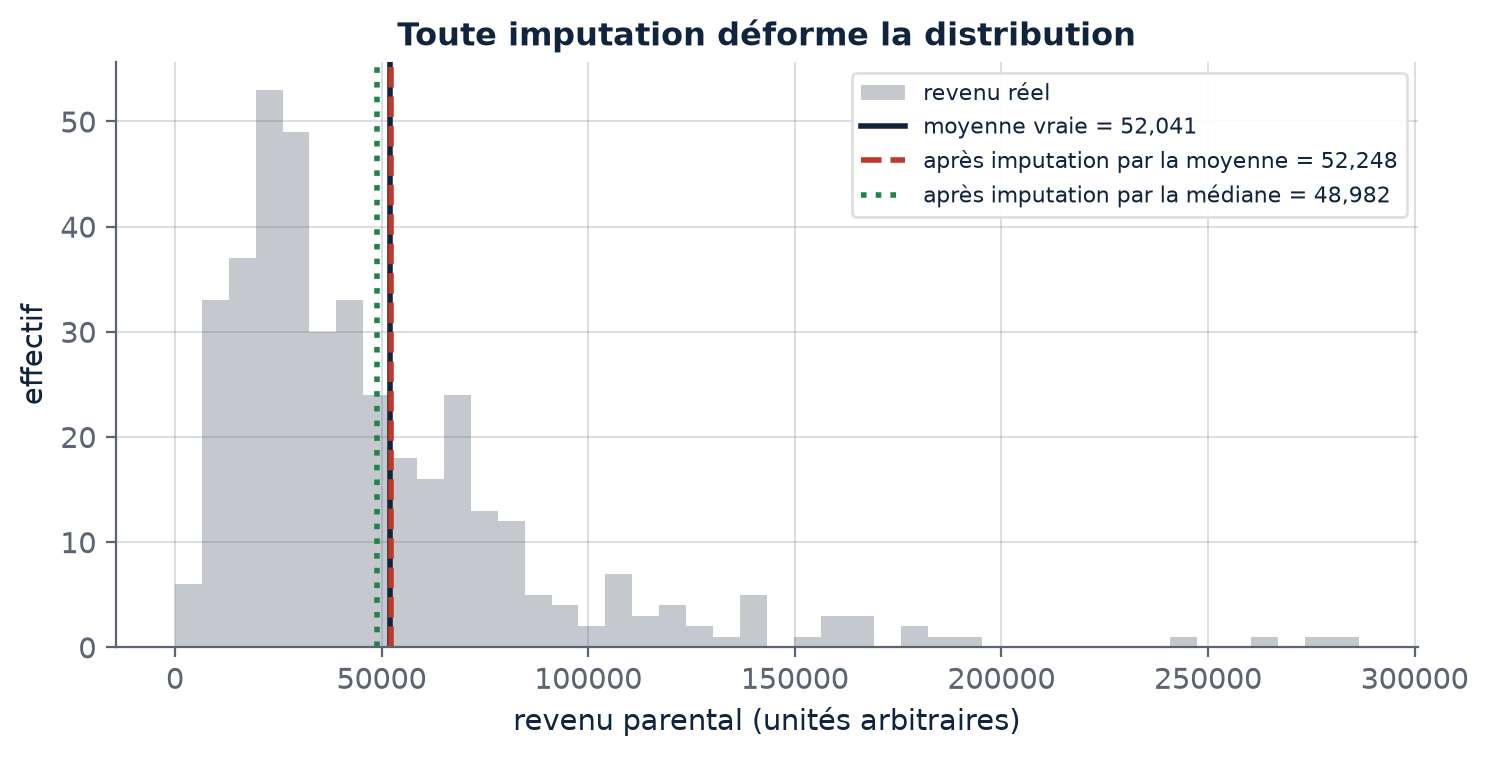
\includegraphics[width=0.86\textwidth]{h02_imputation.png}
\end{center}
\vspace{1mm}
\begin{columns}[t]
\begin{column}{0.48\textwidth}
\footnotesize
\textbf{Moyenne} : $52\,041 \rightarrow 52\,248$ (quasi inchangée), mais
l'écart-type passe de $51\,819$ à $43\,220$, soit \textbf{$-17\,\%$}.
\end{column}
\begin{column}{0.48\textwidth}
\footnotesize
\textbf{Médiane} : la moyenne descend à $48\,982$ ($-3\,059$) : sur une
distribution asymétrique, la médiane n'est pas la moyenne.
\end{column}
\end{columns}
\end{frame}

\begin{frame}{Encoder les catégories}
\begin{center}
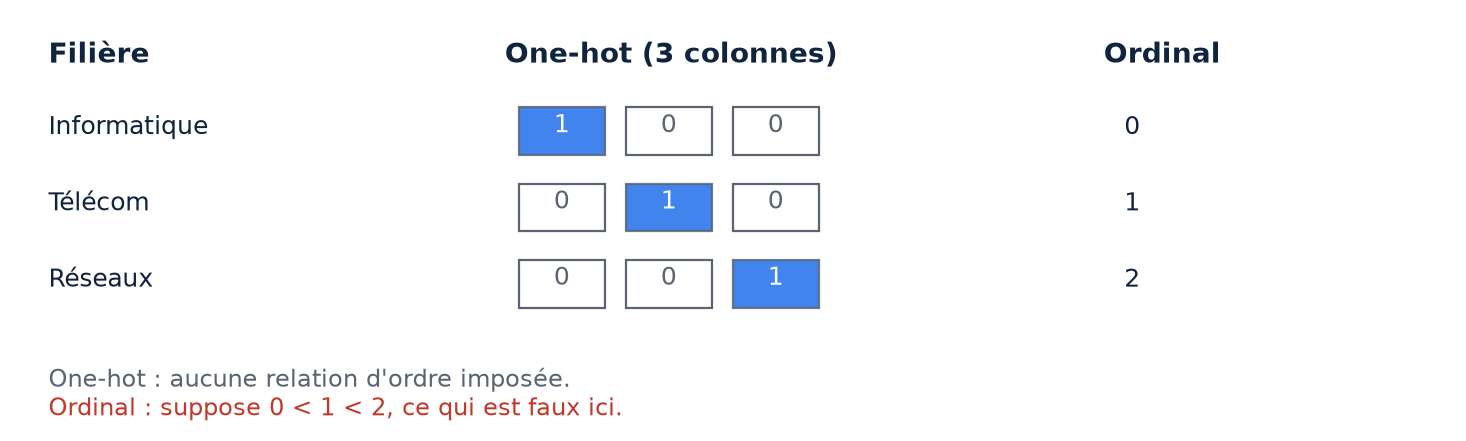
\includegraphics[width=0.92\textwidth]{h03_encodage.png}
\end{center}
\vspace{1mm}
\begin{columns}[t]
\begin{column}{0.32\textwidth}
\begin{ebox}[One-hot]
Une colonne binaire par modalité. Aucun ordre imposé. Coût : $k$ colonnes.
\end{ebox}
\end{column}
\begin{column}{0.32\textwidth}
\begin{ebox}[Ordinal]
Une seule colonne $0,1,2$. À réserver aux modalités \textbf{ordonnées}
(petit / moyen / grand).
\end{ebox}
\end{column}
\begin{column}{0.32\textwidth}
\begin{ebox}[Encodage cible]
On remplace la modalité par la moyenne de $y$. Puissant, mais
\textbf{dangereux} (voir plus loin).
\end{ebox}
\end{column}
\end{columns}
\end{frame}

\begin{frame}{Encodage cyclique : l'heure n'est pas un nombre}
\begin{columns}[t]
\begin{column}{0.46\textwidth}
Une heure va de 0 à 23, puis revient à 0. Encodée telle quelle, 23 h et 0 h
semblent \textbf{très éloignées} alors qu'elles sont voisines.
\[
  h_{\sin} = \sin\!\left(\frac{2\pi h}{24}\right),
  \qquad
  h_{\cos} = \cos\!\left(\frac{2\pi h}{24}\right)
\]
\[
  j_{\sin} = \sin\!\left(\frac{2\pi j}{7}\right),
  \qquad
  j_{\cos} = \cos\!\left(\frac{2\pi j}{7}\right)
\]
\end{column}
\begin{column}{0.50\textwidth}
\begin{kbox}[Pourquoi deux colonnes]
Un seul sinus ne distingue pas 6 h de 18 h. Le couple $(\sin, \cos)$ place
l'heure sur un cercle : la distance euclidienne redevient correcte.
\end{kbox}
\begin{wbox}[Erreur classique]
Encoder l'heure, le mois ou le jour comme un entier. Le modèle apprend alors
une continuité qui n'existe pas.
\end{wbox}
\end{column}
\end{columns}
\end{frame}

\begin{frame}{Activité 1 --- choisir l'encodage (5 min)}
\begin{abox}[Trois colonnes. Quel encodage, et pourquoi ?]
\begin{enumerate}
  \item \textbf{Filière} : informatique, télécom, réseaux (sans ordre).
  \item \textbf{Niveau} : faible, moyen, élevé (ordre naturel).
  \item \textbf{Code postal} : 400 modalités, dont certaines très rares.
\end{enumerate}
\end{abox}
\vspace{1mm}
\begin{solbox}[Réponses]
\textbf{1.} One-hot (3 colonnes).
\textbf{2.} Ordinal (0, 1, 2) --- l'ordre est porteur d'information.
\textbf{3.} Regroupement des modalités rares puis encodage cible \emph{dans les
plis}, ou one-hot avec fréquence minimale.
\end{solbox}
\end{frame}

\begin{frame}{Quiz 1 --- manquants et encodage}
\begin{columns}[t]
\begin{column}{0.49\textwidth}
\begin{qbox}[Question 1]
Imputer par la moyenne conserve :
\begin{itemize}
  \item[(a)] la variance
  \item[(b)] la moyenne, mais pas la variance
  \item[(c)] ni l'une ni l'autre
\end{itemize}
\end{qbox}
\begin{qbox}[Question 2]
Un ordinal convient à :
\begin{itemize}
  \item[(a)] la filière
  \item[(b)] le niveau faible/moyen/élevé
  \item[(c)] le code postal
\end{itemize}
\end{qbox}
\end{column}
\begin{column}{0.49\textwidth}
\begin{qbox}[Question 3]
Pourquoi encoder l'heure en $(\sin,\cos)$ ?
\begin{itemize}
  \item[(a)] pour réduire le nombre de colonnes
  \item[(b)] pour respecter la continuité circulaire
  \item[(c)] parce que le modèle l'exige
\end{itemize}
\end{qbox}
\begin{solbox}[Réponses]
\textbf{1.} (b). \quad \textbf{2.} (b). \quad \textbf{3.} (b).
\end{solbox}
\end{column}
\end{columns}
\end{frame}
